%!TEX root = ../Thesis.tex

\def\chapdir{./ChapterLiteratureReview}

\chapter{Literature Review} \label{ch:litreview}



%\section{Position Requirements}
%- how/why to use position for applications\\
%- absolute vs relative\\
%- why use relative positioning\\
%- knowing where you are positioned is important for data gathering, motion detecting and tracking, path planning\\
%- formation flying, drones\\
%- data fusion, needed for drift correction

%\section{GNSS Introduction} % just have as intro to the lit review?
%America with GPS and Russia with GLONASS are at the time of writing the only two fully functional GNSS constellations. The EU and China are developing their own constellations called Galileo and Beidou respectively.

Global Navigation Satellite System (GNSS) is a generic term for a satellite navigation system that provides autonomous localisation and tracking on a global scale. Some countries have developed or in the process of developing their own GNSS. This thesis focuses on the American GPS (Global Positioning System) due to information accessibly and extensive usage in literature as it is the oldest constellation.

\begin{figure}[!h]
\centering
\caption{GPS Constellation in Earth-Centered Inertial frame}
\label{fig:GPS_ECI_side}
\begin{subfigure}[t]{0.49\linewidth}
\centering
\caption{Side View}
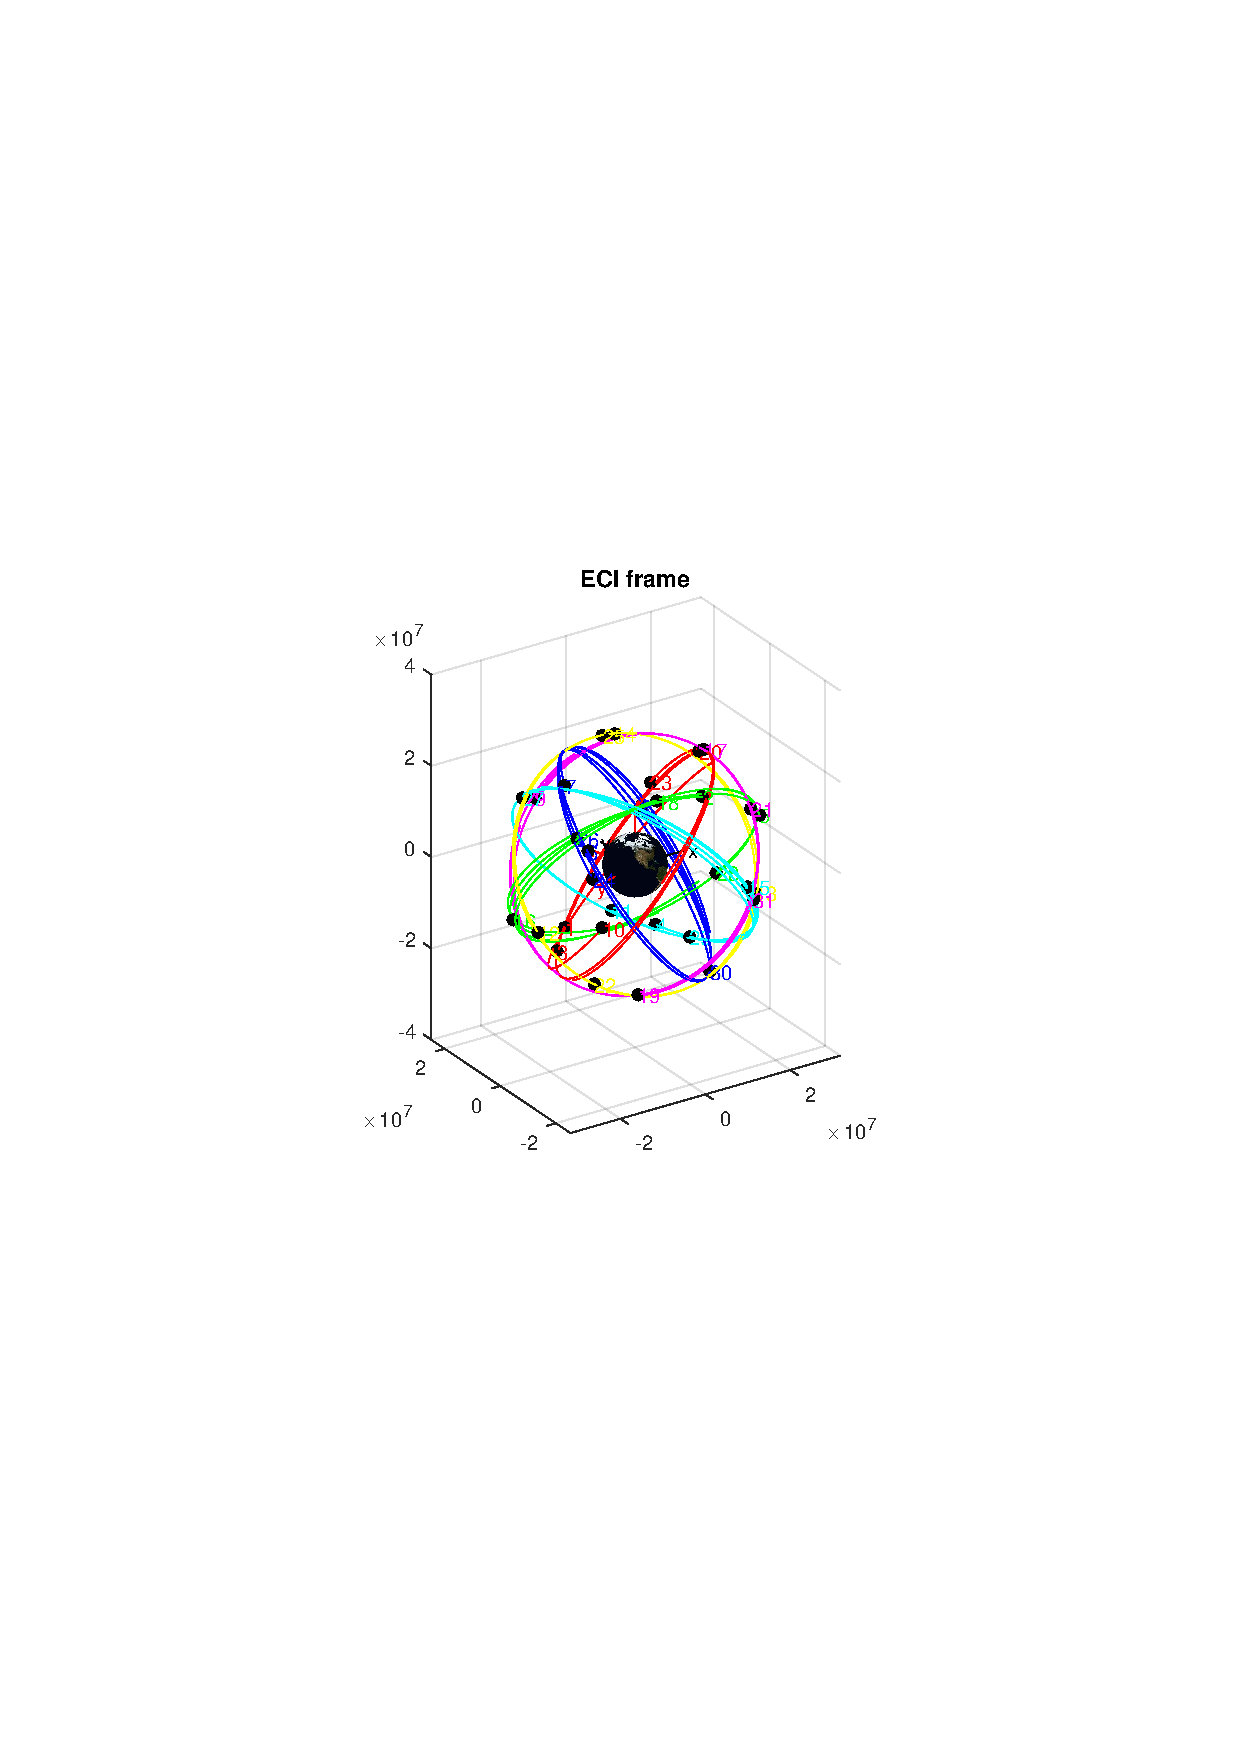
\includegraphics[trim=6cm 9.5cm 6cm 10cm,clip,width=0.8\linewidth]{ChapterLiteratureReview/GPS_ECI_side}
\end{subfigure}
\begin{subfigure}[t]{0.49\linewidth}
\centering
\caption{Top View}
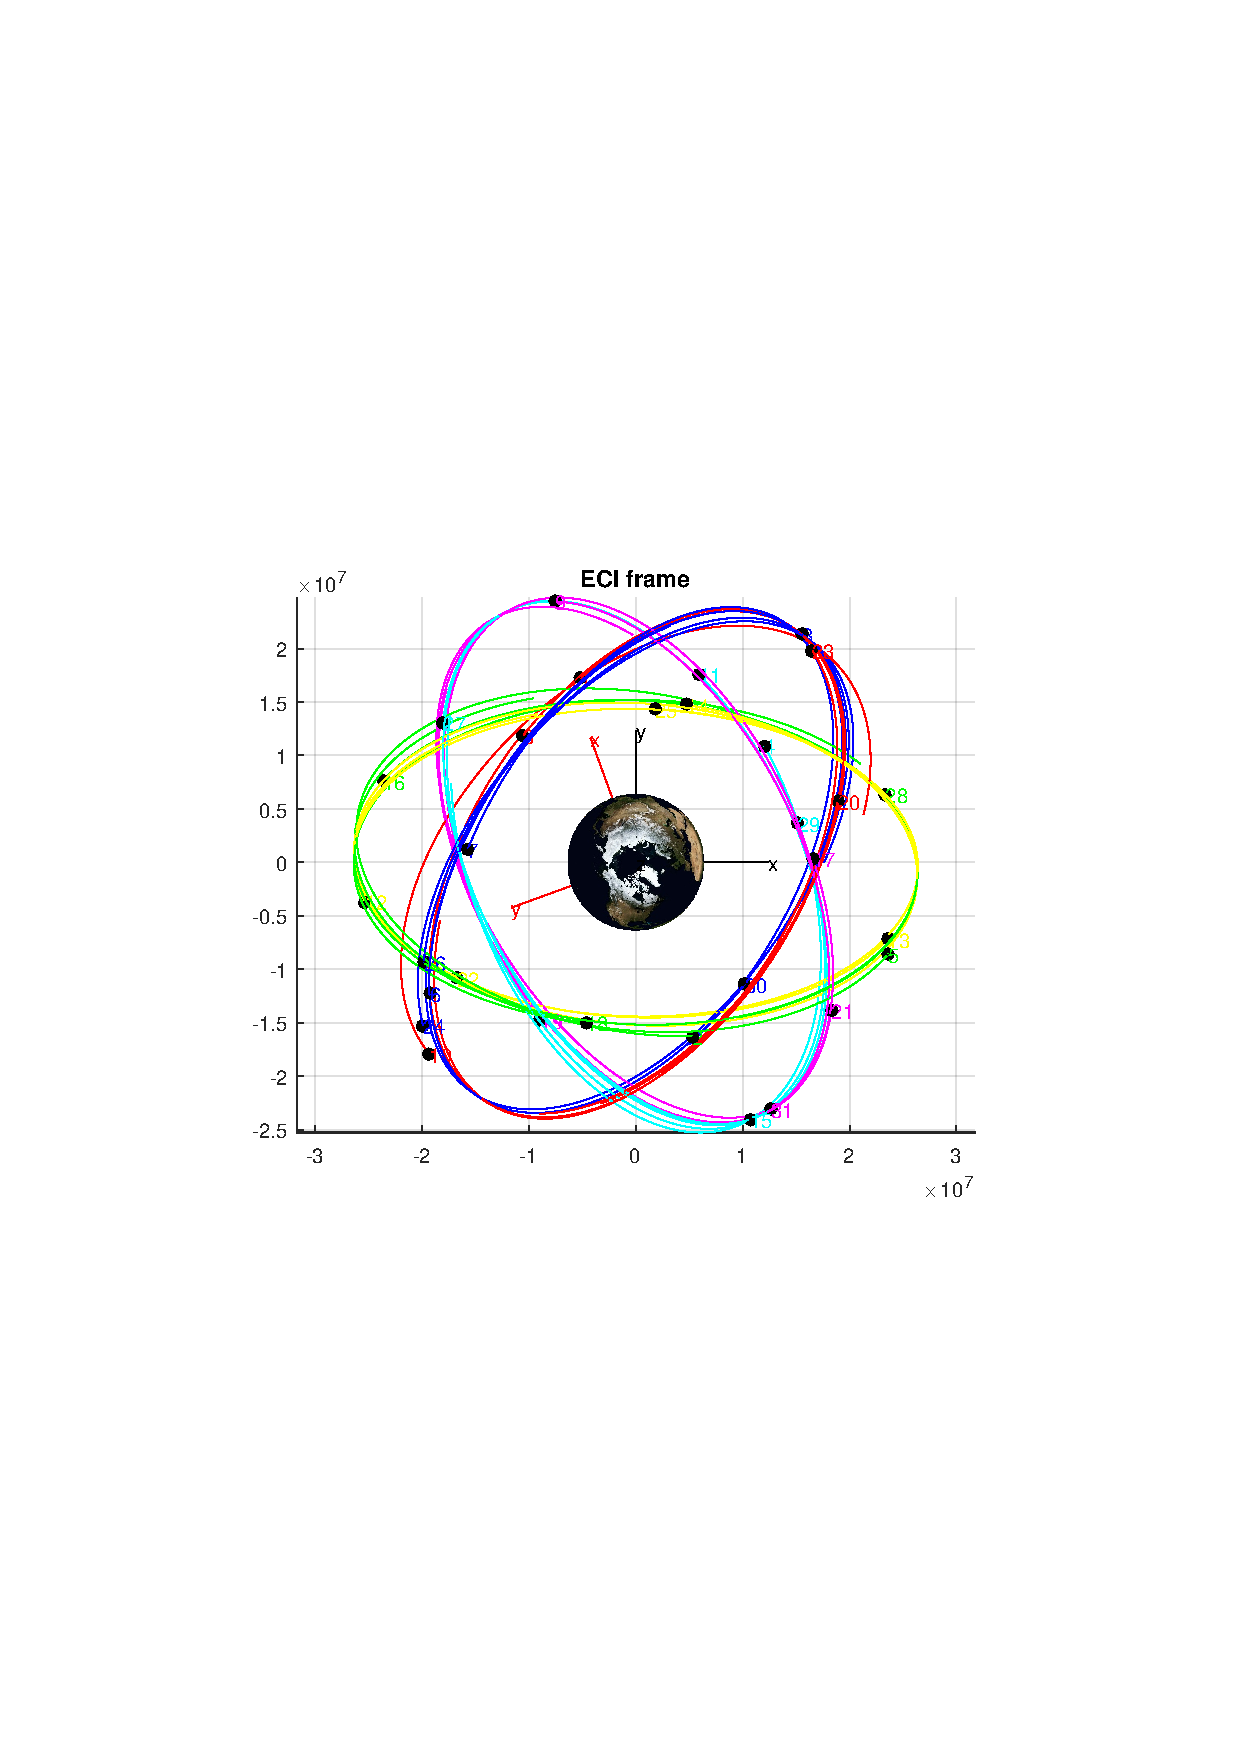
\includegraphics[trim=4cm 10cm 4cm 9cm,clip,width=\linewidth]{ChapterLiteratureReview/GPS_ECI_top}
\end{subfigure}
\end{figure}

%\begin{table}
%\centering
%\caption{GNSS Constellations}
%\label{Table:gnss constellations}
%\begin{tabular}[width=\linewidth]{|l|l|c|c|c|}
%\hline
%Country & Name & Number of Satellites & Start Date & End Date \\\hline
%America& GPS & 31 & &  \\\hline
%Russia & GLONASS & 24 & 1976 &  \\\hline
%European Union& Galileo &  & 1998 & \\\hline
%China & Beidou & & &  \\\hline
%\end{tabular}
%\end{table}

%!TEX root = ../Thesis.tex


\section{GPS Operational Components}
There are three components to the whole GPS system; the space segment, the user segment, and the ground control segment. The satellite sends radio signals towards the Earth which is received by both users and ground control centers. The ground control tracks the satellite and the data to analyse the satellite parameters and returns periodic updates to the satellite about its status. The satellite then updates its signal to the new parameters. The user receives the signal from the satellite with the updated parameters.

\subsection{Space Segment}
- current GNSS: explain GPS, GLONASS, galelao, chinese one constellations and how it works
- what orbits are they in and why?: altitude\\
inbetween the two radiation belts?

The GPS constellation consists of 32 operational satellites in six different orbital planes



\subsection{User Segment}
The user is a passive participant in the GPS system.
- typical accuracy for civilian accessable gps\\
- military has more precise stuff\\
- lower cost receivers have only one frequency band, error in timing\\
Unfortunately, low cost GNSS receivers rarely provide official access to the GPS raw data. Previous studies have used customised bluetooth headsets or customised android platform mobile phones to investigate algorithms on low-cost GPS receivers. More expensive receivers do allow raw data to be utilised, however they also provide other mechanisms such as duel frequencies and more accurate clocks, rendering the new algorithm *obtuse*. The mindset of *crowd-sourcing*/customising/flexible technology is changing the way manufactures build GPS receivers. The new Android OS platform Nougat 7.0 provides the developer raw GPS data at the software level.  

\subsection{Ground Control Segment}
On the ground spread all over the world, are control stations that monitor the satellites. 
- tracking -> distance and angle - active as it sends back information
-Locations of control stations and why they're there

Uses Herrick-Gibbs algorithm to determine the orbit of the satellite. A satellite is tracked over a ground station for a period of time and its position is measured. From three position vectors the velocity vector can be calculated and the ephemeris parameters are estimated. The ephemeris parameters describe the orbit of the satellite and are used to calculate the position of the satellite at any point in time by the user segment. The time parameters and clock corrections of the satellite are also calculated by the ground control station and sent back in the navigation message.
The ephemeris data is highly accurate and updated every two hours.






%!TEX root = ../Thesis.tex

\section{GPS Satellite Signals} \label{sec:signals}
The are two frequencies that GPS uses; L1 frequency at 1575.42 MHz and L2 at 1227.60 MHz \cite{signal spec}. There are two sets of signals that are sent from every satellite, the pseudorandom binary sequence (PRN code) and the navigation message.

\subsection{PRN}
Coarse Acquisition Code, or C/A code, is transmitted on the L1 frequency as a 1.023 MHz signal of 1023 bits. Civilians have access to the C/A code and is what is used in receivers. There is another code modulated onto the L1 and L2 frequencies called the P (Precise) code as a 10.23 MHz signal \cite{CA_oxts}. As it is 10 times faster it is more accurate, and is restricted to military use. Both of these codes are modulated as pseudo random number (PRN) codes and repeat constantly, which have the property of the appearance of random noise but are very precisely defined. It is because it is precisely defined, the GPS receiver can recreate the PRN code at the same time the satellite does. By comparing the incoming signal and the self-generated code the time delay is measured, see Figure \ref{fig:PRNtime}. As the C/A code repeats every millisecond, only a time range of 1 ms needs to be searched \cite{trimble_PRN}.


\cite{mit_signals}

\begin{figure}
\centering
\caption{Pseudorange measurement from the time delay of the PRN code \cite{whatwhenhow}}
\label{fig:PRNtime}
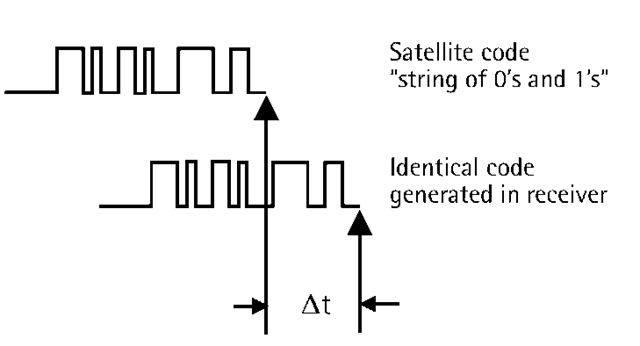
\includegraphics[width=0.7\linewidth]{ChapterLiteratureReview/PRNtime.png}
\end{figure}



\subsection{Navigation Message}
The navigation message is a low frequency signal added to the L1 code at a rate of 50 bps. It has three components \cite{signalspec};
\begin{enumerate}
\item GPS date and time with satellite status at the time the signal was sent
\item Ephemeris data: valid for up to 4 hours
\item Almanac data: valid for 180 days
\end{enumerate}
The almanac data 


\begin{figure}
\centering
\caption{Navigation Message Content and Format Overview \cite{signalspec}}
\label{fig:NavMessage}
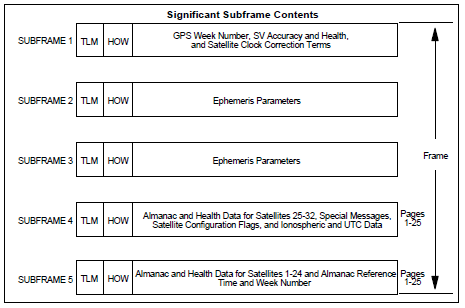
\includegraphics[width=0.7\linewidth]{ChapterLiteratureReview/NavMessage}
\end{figure}



\subsection{Raw Data}
There is a lot of data contained in the total signal, but the following are what is important to this thesis:
\begin{itemize}
	\item \textbf{Time received}: The time in the receivers frame that the sample reading was taken.
	\item \textbf{Pseudorange}: The range calculated by the receiver to the satellite. Depending upon the type of receiver, this measurement may have already been adjusted for some errors that were encoded in the navigation message.
	\item \textbf{Carrier Phase}: The phase of the carrier signal at the receivers point in time.
	\item \textbf{Doppler Shift}: The instantaneous Doppler frequency of the signal. 
	\item \textbf{Satellite Epoch}: The time the signal was sent from the satellite, decoded from the navigation message.
	\item \textbf{Ephemeris Data}: The orbital parameters necessary to calculate the position of the satellite.
\end{itemize}


%The first row shows a C/A code with 1,023 chips; the total length is 1 ms. The second row shows a navigation data bit that has a data rate of 50 Hz; thus, a data bit is 20 ms long and contains 20 C/A codes. Thirty data bits make a word that is 600 ms long as shown in the third row. Ten words make a subframe that is 6 seconds long as shown in row four. The fifth row shows a page that is 30 seconds long and contains 5 subframes. Twenty-five pages make a complete data set that is 12.5 minutes long as shown in the sixth row. The 25 pages of data can be referred to as a superframe http://read.pudn.com/downloads85/ebook/326017/Fundamentals%20of%20Global%20Positioning%20System%20Receivers/booktext05.pdf (pg77)

% resources about the signals:
% http://geoconnect.com.au/gps-signals-l1-l2-l5/
% http://www.trimble.com/gps_tutorial/dgps-advanced4.aspx
% https://www.e-education.psu.edu/natureofgeoinfo/c5_p14.html
% http://what-when-how.com/gps/gps-details/
% https://www.e-education.psu.edu/geog862/node/1742
% http://indico.ictp.it/event/a09138/session/24/contribution/14/material/0/0.pdf
% http://read.pudn.com/downloads85/ebook/326017/Fundamentals%20of%20Global%20Positioning%20System%20Receivers/booktext05.pdf
% http://www.navipedia.net/index.php/GPS_Navigation_Message

%!TEX root = ../Thesis.tex

\section{Trilateration}
Unlike triangulation, which uses the angles from known points, trilateration uses the distances from known points. This is the base concept behind GNSS. Satellite W sends out a radio signal at time X and it's position Y which the user received at time Z. The time difference is used to calculate the distance from the satellite's position, see Figure \ref{fig:trilateration}. With this information from multiple satellites, the users position is calculated. In reality, the distance from the satellite to the user has error in it, which will be explained in detail in Section \ref{sec:error sources}. The error alters the radius of the circle (or in 3D the sphere), see Figure \ref{fig:trilaterationtime}. The error is expressed as a clock bias, a change in time at the receiver side in order to find an intersection. As there are four variables to solve for, x, y, z and clock bias $b_u$, a minimum of four satellites are required to calculate the intersection. The range that has error in it is called the pseudorange.
\begin{figure}
\centering
\caption{Solve for Position using Trilateration}
\label{fig:trilateration}
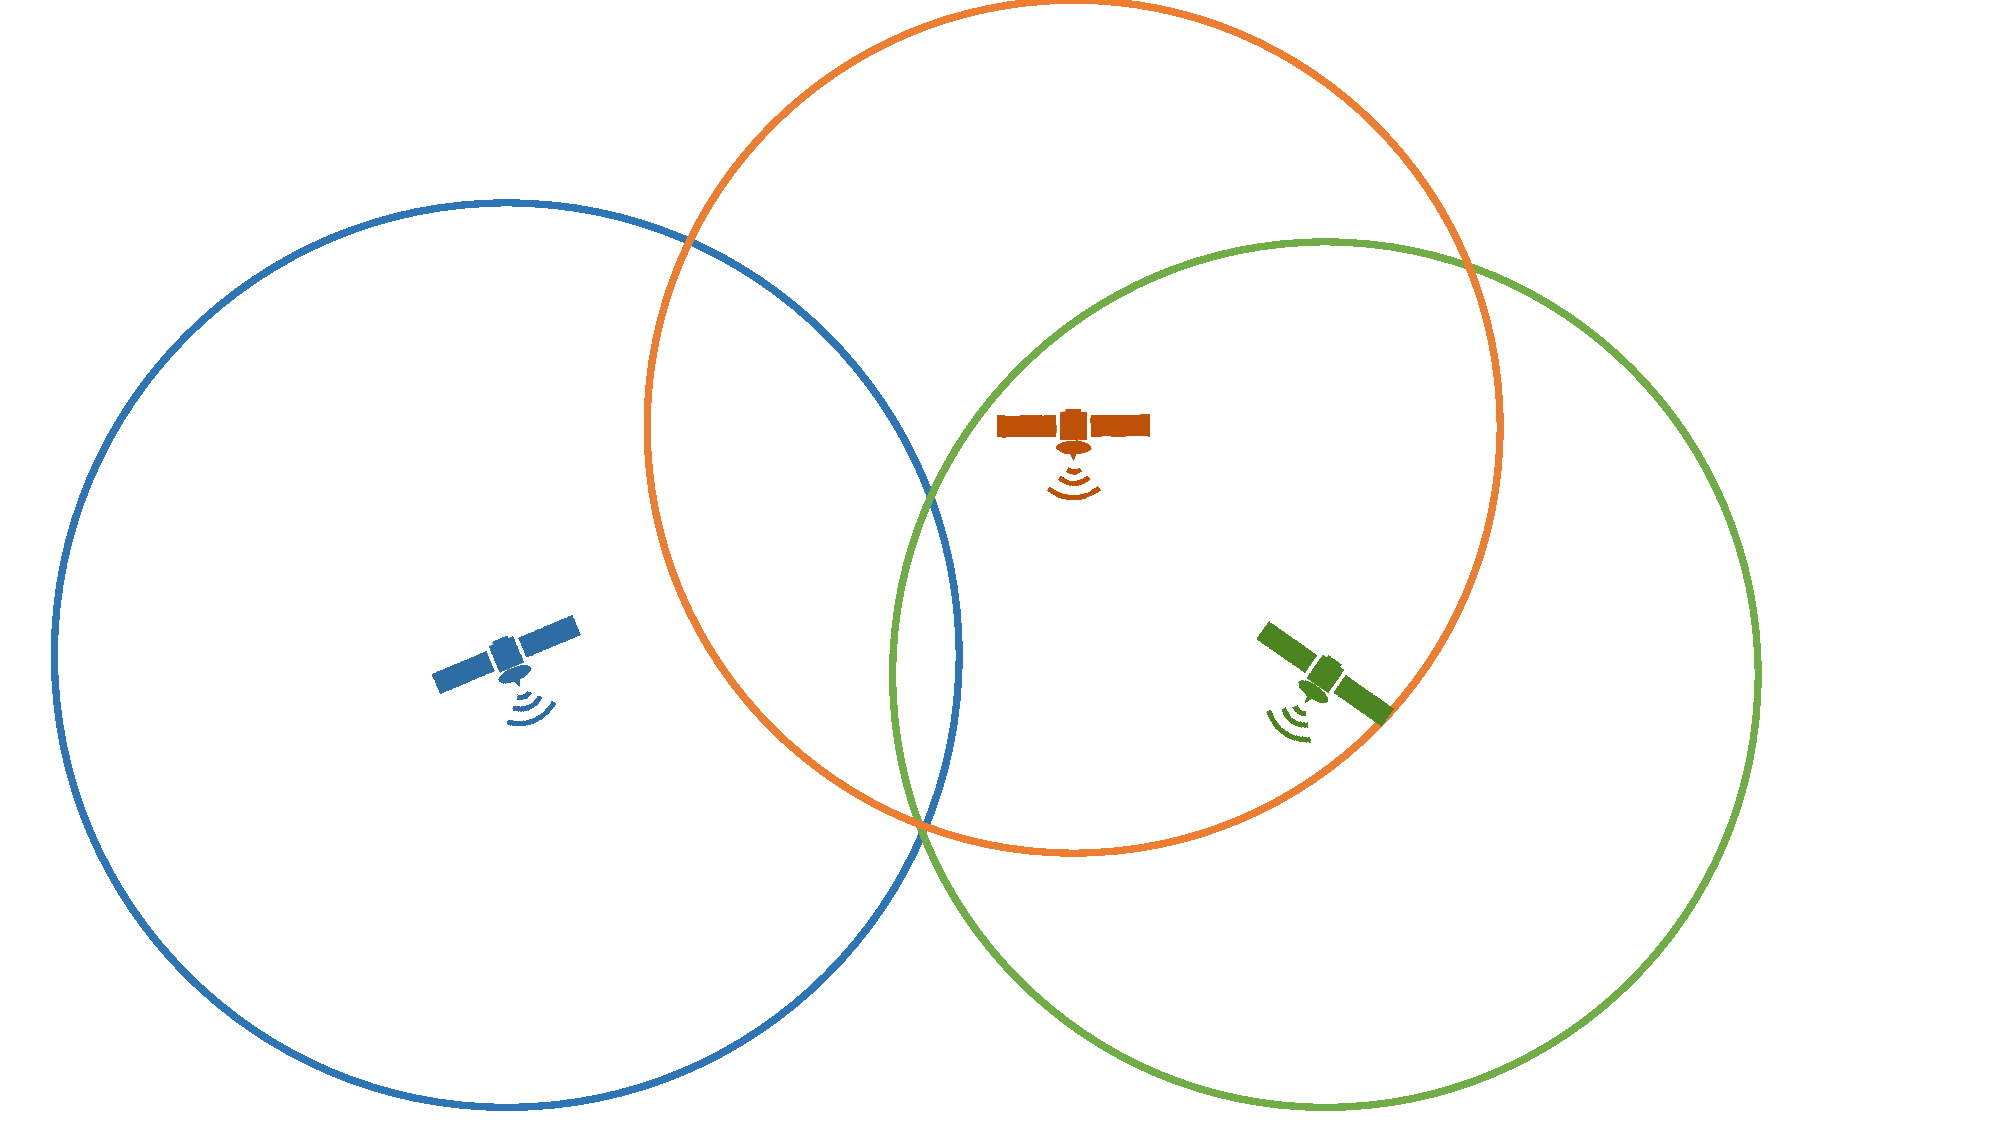
\includegraphics[width=0.7\linewidth]{ChapterLiteratureReview/trilateration}
\end{figure}
\begin{figure}
\centering
\caption{Solve for Position and Clock Bias using Trilateration}
\label{fig:trilaterationtime}
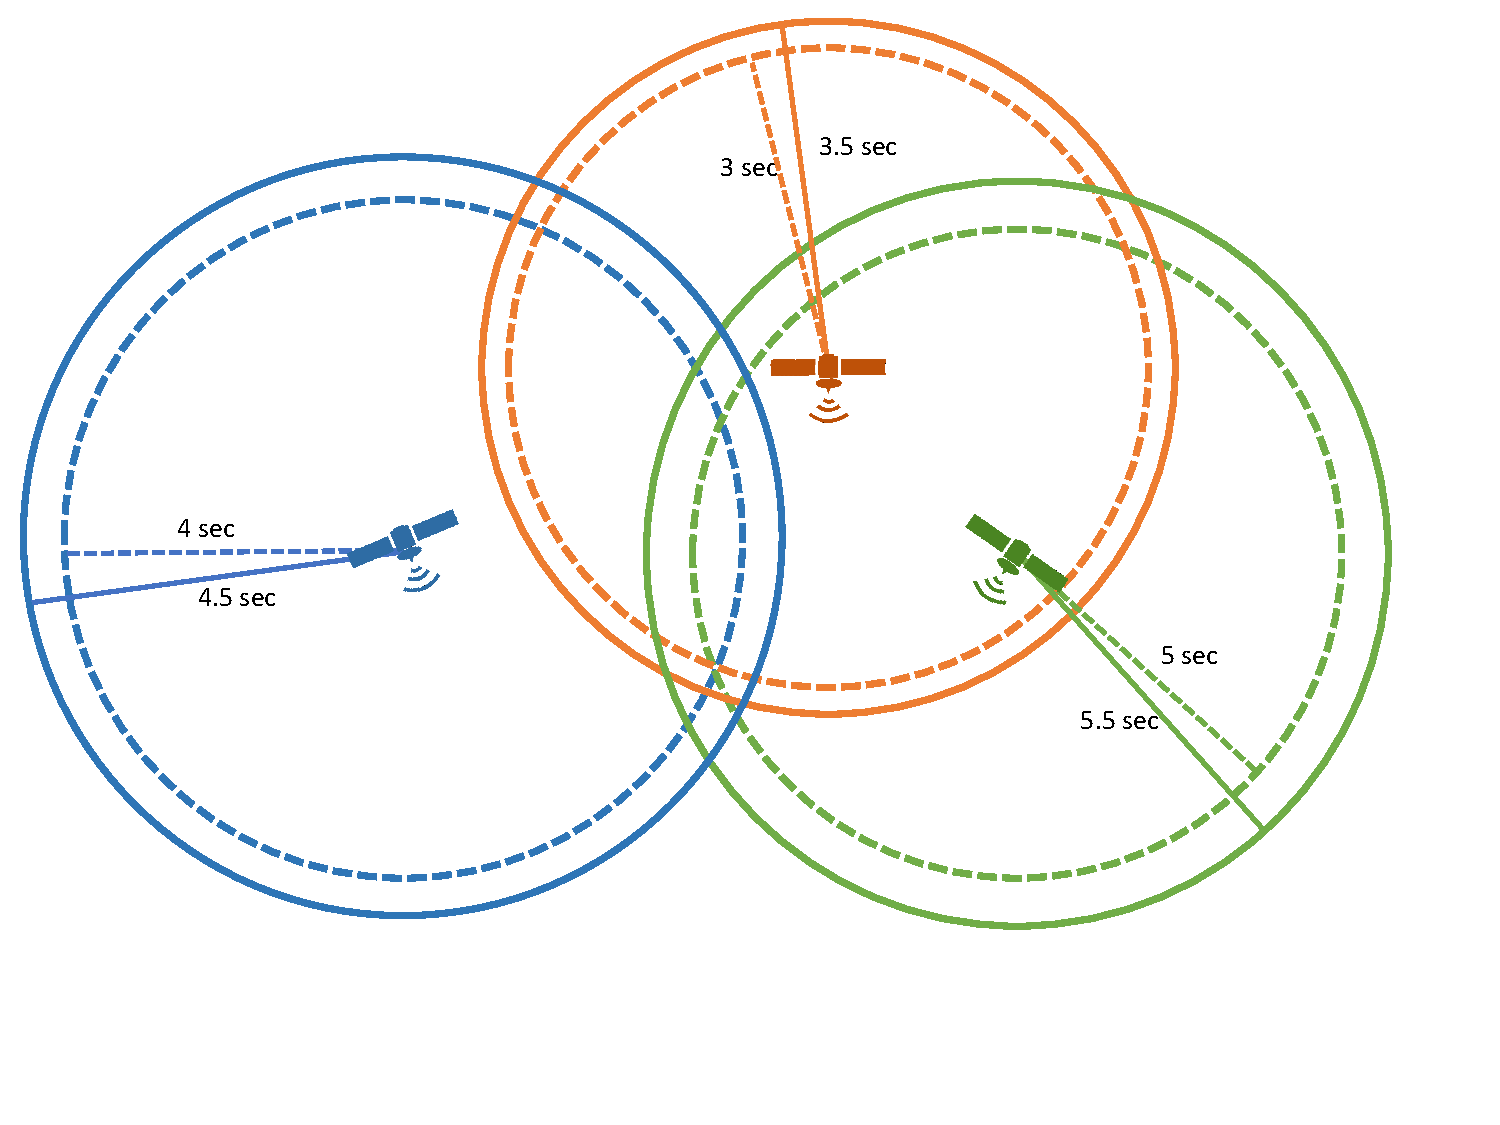
\includegraphics[width=0.7\linewidth]{ChapterLiteratureReview/trilaterationtime}
\end{figure}

\subsection{Nonlinear Least Squares} \label{sec:NLLS}
There may be more than four satellites in view, which creates an overdetermined system. There is not exact solution when the system has error, so it is solved via non-linear least squares (NLLS).
\begin{eqnarray}
\rho_i = \sqrt{(X_{SV_i}-x)^2+(Y_{SV_i}-y)^2+(Z_{SV_i}-z)^2} +cb_u + \epsilon
\end{eqnarray}
Where $\rho_i$ is the pseudorange of the receiver to satellite i, [$X_{SV_i},Y_{SV_i},Z_{SV_i}$] is the position of the satellite i, c is the speed of light, and $\epsilon$ is some measurement noise. NLLS is a standard algorithm that linearises about an estimate of the state variable
\begin{enumerate}
\item Assume an initial estimate of the system state
\item Linearise the system about the estimate by calculating the Jacobian
\item Calculate the residual between the estimated location and the measured ranges
\item Identify the residual due to the linearised system
\item Minimise the quadratic error to calculate the best linear step
\item Update the estimate using the linear step
\item Repeat until convergence
\end{enumerate}






- NLLS solve spheres

- ECEF frame of reference

%!TEX root = ../Thesis.tex

\section{GPS Error Sources} \label{sec:error sources}
There are many sources of error that plague the GPS data. These errors are categorised into six types; multipath, atmospheric effects, receiver noise, ephemeris error, clock bias and Sagnac effect.

\subsection{Mutlipath Interference}
Multipath is the case where the radio signal is reflected off objects before reaching the receiver, which increases the distance travelled. It is especially prevalent in built-up areas with tall buildings. 

\subsection{Atmospheric Effects}
The distance from a satellite to a user is calculated by the time difference when the radio signal was sent and when it was received multiplied by the speed of light. However, the speed of light is reduced when in the atmosphere compared to that in space.
The ionosphere is the upper layer of the atmosphere ranging from 50 to 500 km. It consists of ionized particles that create fluctuating electric fields in the atmosphere that perturb the radio signals that travel through it. This effect can be modelled but is still a significant source of error, approximately 5 m \cite{trimble_errors}. The troposphere is the lowest part of the atmosphere up to 50 km that varies in temperature and pressure with weather patterns. The radio signals are refracted through the medium, but as it is only for a short period of time this error is significantly less than that of the ionosphere at approximately 0.5 m error \cite{trimble_errors}.

\subsection{Receiver Noise}
In any electronic components, especially low cost components, thermal noise introduces error into the system. Thermal noise is caused by the random motion of electrons in conducting materials. The construction of the electrical components are not identical, which also cause slightly different solutions from receiver to receiver. This can contribute approximately 0.3 m of error \cite{trimble_errors}.

\subsection{Ephemeris Error}
The ephemeris error is the error in the navigation data describing the orbital parameters of the satellite \cite{Kaplan_ephemeriserror}. This information is approximated and updated every 2-4 hours by the control segment to minimise the error. The approximation is based on a prediction model of the orbital parameters, as there are many forces that act on a satellite that can alter the orbit. These include gravitational affects of other masses in the solar system such as the Moon, the Sun, even Jupiter and the outer planets affect the gravitational potential of objects in orbit around Earth. The non-spherical Earth, solar radiation pressure, slight atmospheric pressure are all forces that manipulate the orbit. The satellites also undergo station keeping manoeuvres to manage the orbit, which the requires the ephemeris data to update. This inaccuracy contributes about 2.5 m in error \cite{trimble_errors}.

\subsection{Clock Bias}
The clock on the satellites and receivers are not exact with the true GPS time. Low-cost receivers are built with cheap quartz crystal oscillators that keep time to $1\mu s$ accuracy. The clocks on the satellites however are atomic clocks that have accuracy on the order of $1 ns$. In addition to this, ground control can measure the satellite clock bias and send back that information to be stored in the navigation message. \cite{zinas_2015}

\subsection{Sagnac Effect}
The sagnac effect is a more intrinsic source of error. It is due to the rotation of the Earth during the time of the signal transmission. The transmission time is between 0.06-0.08 seconds in which time the Earth has rotated approximately 30 m. If the ephemeris data was in an inertial frame (ECI) there would not be a problem. However, the data is in the Earth-Centred Earth-Fixed (ECEF) frame which is a frame that rotates with the Earth to allow users to calculate their positions independent of time \cite{HighAccDiffTrack}.

\subsection{GPS Error Summary}
All of the errors mentioned above can be categorised into three types; satellite correlated, receiver correlated, and uncorrelated errors. That is, a particular type of error may be consistent between all receivers from a particular satellite, or consistent between all satellite measurements for a particular receiver, or neither. See Table \ref{Table:error catagory}.

\begin{table}
\centering
\caption{Categorisation of Errors}
\label{Table:error catagory}
\begin{tabular}{|c|c|c|}
\hline
Satellite & Receiver & Uncorrelated \\\hline
satellite clock bias & receiver clock bias & multipath \\
ionospheric delay & receiver noise& Sagnac \\
tropospheric delay & &  \\
ephemeris error & & \\\hline
\end{tabular}
\end{table}

 % DONE

%! TEX root = ../Thesis.tex


\section{Multiple Receivers}
- problems arising with multiple receivers

A single sample of pseudoranges from any two receivers will not be taken at the exact same time without a connecting network to implement control. This means that the satellite positions at the time of each signal transmission will be actually different. The primary issue with calculating the change in pseudorange is identifying the transmission time 


\subsection{Align Reception time}
In \cite{HighAccDiffTrack}, they align the reception time of multiple receivers

They precisely align the epoch by accounting for the differing Sagnac effect between two receivers and accounting for the clock biases of the receivers. The Sagnac effect manifests in the multiple receivers case by the signal propagation time for a measurement taken at $t_2$ would be different than if it was taken at $t_1$, the Earth will have rotated by different amounts. 
\begin{enumerate}
\item The clock bias is calculated by solving for the individual absolute position of a receiver using least squares. This is necessary in order to 
\item  
\end{enumerate}

%!TEX root = ../Thesis.tex

\section{Current GNSS algorithms}
- just reference implementation papers?
- algorithms to make it more accurate\\
- use for motion tracking\\
- performance vs cost trade off\\
(http://ieeexplore.ieee.org.ezproxy1.library.usyd.edu.au/document/7530542/)

\subsection{Standard Positioning Service}
The Standard Positioning Service (SPS) is the default system that provides PNT signals as described in Section \ref{sec:signals} for free to civilian, commercial and scientific uses worldwide. It has been operational since 1993 and has minimum performance commitments of 3 meters horizontal accuracy and 5 meters vertical accuracy as of 2007 which was the latest edition of the Performance Standard USA Department of Deference issued \cite{officalperformance}. The GPS receivers use trilateration and solve for position and time with NLLS algorithm as described in Section \ref{sec:NLLS}. 

- single frequency and multi frequency to remove atmospheric affects

Currently the DOD is 
code phase

\subsection{Carrier Phase Solution}


\subsection{Duel Frequency Precise Point Positioning (DF-PPP)}
The ionospheric delay is one of the largest sources of error in the system. The electrical interference is diffusive, and is dependent on the frequency of the signal. The two signals are used to remove the ionosphere delay then combined to solve for the carrier phase ambiguities. This system can produce centimeter or decimeter accuracy but requires 20-40 minutes to converge to that accuracy. Also the duel frequency receiver costs more than single frequency receivers \cite{gnsssolutions_dfppp}.


\subsection{Differential GPS}
Differential GPS (DGPS) is a way to correct satellite correlated errors by using a stationary receiver in a well known location. It ties the satellite measurements into a local reference by solving for the reference receiver's position in reverse. That is, it solves for the timing errors in the satellite signal as it knows what position it should be in. The stationary reference receiver then broadcasts the error correction information to any roaming receiver in its vicinity. 


- explain what it is\\
- what setup is required \\
- abs vs rel \\
- degree of accuracy
\subsection{WAAS DGPS}



\subsection{Post Processing Algorithm}

\subsection{Single Frequency Precise Point Positioning (SF-PPP)}
Rademakers \textcolor{red}{how to say reference?} at University of Delft in the Netherlands developed a solution for finding the absolute position in open areas to a horizontal accuracy of 0.5 m. It uses a single frequency, single antenna low cost GPS receiver by connecting to the internet and using real time information to model all errors. The errors they corrected with the potential improvements are outlined in Table \ref{Table:SFPPP error table}. 
\begin{table}
\centering
\caption{Error Components and Potential Improvements for SF-PPP}
\label{Table:SFPPP error table}
\begin{tabular}{|l|l|}
\hline
\textbf{Error component} &\textbf{ Potential Improvement} \\\hline
 Ionosphere: Klobuchar model & 7 m \\\hline
 Troposphere: Saastamoinen model & 2.5 m \\\hline
Ephemeris data &  1 m \\\hline
 Satellite clock drift & 1.5 m \\\hline
 Differential code bias & 50 cm \\\hline
 Phase windup: rotation of the antenna & dm \\\hline
 Sagnac effect & 30 m \\\hline
 ROA: satellite orbit correction & up to 10 cm \\\hline
 Relativistic clock correction & up to 21 m \\\hline
 Moon-Earth interaction & 5cm (Hor) and 30 cm (Ver)\\\hline
\end{tabular}
\end{table}


\subsection{Duel-Epoch, Double-Differencing Model} \label{DEDD}
In the paper by the Institute of Software Integrated Systems, Vanderbilt University called \textit{High-Accuracy Differential Tracking of Low-Cost GPS Receivers}, Hedgecock and party developed a new algorithm for relative motion tracking for multiple receivers. They used low cost GPS receivers with access to raw measurement data to produce centimeter-scale tracking accuracy. Each receiver was shared the whole networks data and ran the localisation algorithm independently to avoid having a single point of failure.\\

The algorithm uses the change in carrier phase through time of each receiver to estimate the change in relative ranges between a satellite and two receivers. It does not require a reference satellite, a reference node or an integer ambiguity solution. It does require the clock bias for each receiver at each point in time as solved for by non-linear least squares for the absolute position before running the algorithm itself. To reiterate, it does not directly solve for the relative position but the relative motion. However, neither of the initial positions of the receivers need to be precisely known in order for the relative motion to be accurate. Due to the time dependency, consistent satellite locks of at least four satellites are required, otherwise reinitialisation must occur. The calculated change was projected onto the unit direction vector from receiver to satellite. The system of these tracking equations was solved via least squares optimisation. \\

It uses the assumption that all satellites in the constellation are such a great distance from the surface of the Earth that the unit vector from both receivers are parallel to each individual satellite, as long as it is in the same geographical region. How far apart the receivers can be for this assumption to hold was not stated.\\ 




- how many receivers?\\
- why and how it aligns epoch\\
- uses difference in time for a single receiver to find change in motion.



- have this one last as it is the most similar\\
- needs instantaneous relative distance for first point, to speed up processing and make the first few time steps more accurate, also when locking onto new satellites


\subsection{Summary of Algorithms ?}

% types of algorithms making gps more accurate: table with columns = types of analysis, rows= types of algorithms
- dynamic tracking (need temporal measurements) vs static measurement - no temporal\\
- post processing vs pre-processing vs realtime\\
- ground structure vs free standing\\
- absolute vs relative\\
- accuracy (how much)\\
- computation time/space required\\
- what error is each method removing\\
- what piece of data it needs (if raw)\\
- calibration required\\
- robustness -> if a satellite goes out of view does it need to re-calibrate? passing information between receivers-> is one a reference? single point of failure





%!TEX root = ../Thesis.tex

\section{Moving Forward} % or is it conclusion?
GPS is currently going through a major upgrade, with the launch of new satellites with alternate structuring of signals that will provide greater accuracy for civil use in the future. The constellation Galileo that is currently being developed and launched, is expected to be finished by XX. Both the new GPS and Galileo are designed to be able to operate in tandem to provide an *unprecedented* accuracy with a total of 57 operational joint satellites, while still having the individual capability of global coverage. Some technology today uses both GPS and GLONASS constellations but requires duel receivers as the signals are encoded differently. GPS uses code division multiple access (CMDA) whereas GLONASS uses frequency division multiple access (FMDA). Research is also being conducted on the sources of error in the radio signals. The errors are to be modelled and the appropriate adjustments stored in the encoding of the signal. Through the international cooperation efforts and research, localisation and tracking using baseline GNSS will continue to improve, regardless of alternate data processing algorithms. For now, improved signal accuracy will obviously improve the performance of the different data processing algorithms. However, there will come a time where the extra computational and hardware complexity will not be worth the small gain in accuracy over the default performance of the low-cost civilian GNSS receiver.
 % DONE








%??Topical organisation with inverted pyramid substructure
% \subsection{GNSS Localisation}
% Global Navigation Satellite System (GNSS) 
% - lower update rates $\approx$1Hz\\
% - accuracy/precision? not good enough for these applications\\
% - not good for indoor environments as signals are weak\\
% - used differentiated gnss to solve for integer ambiguity across multiple mobile platforms on the go \cite{GNSS_difftrack} \cite{GNSS_intamb}\\
% - multipath/atmospheric error estimation \\
% - multiple receivers across the multiplayers \cite{GNSS_multi} \\

% 	%% types of precision gnss locations 
% - double differentiating - requires same satellites
% - pvt position velocity and precise time